\pdfoutput=1
\documentclass[12pt]{article}

\usepackage{amsmath, amssymb, amsthm}
\usepackage{graphicx}
\graphicspath{{../}}
\usepackage{booktabs}
\usepackage{array}
\usepackage[colorlinks=true, linkcolor=blue, citecolor=blue, urlcolor=blue]{hyperref}
\usepackage[numbers,sort&compress]{natbib}
\usepackage{geometry}
\geometry{margin=1in}

\theoremstyle{remark}
\newtheorem{remark}{Remark}[section]
\newtheorem{observation}[remark]{Observation}

\title{Phase-Resolved Transparency Classification in Commodity Supply Chains:\\
        \large A Structural Triadic Scoring Framework (TVPCI)}
\author{Jeffrey W. Milton\\\\[4pt]\small Clarity Coalition}
\date{2026}

\begin{document}
\maketitle

\begin{abstract}
Opacity in commodity supply chains is commonly described in narrative or intent-based terms.
This paper proposes a structural alternative: transparency is a property of
\emph{observable evidence attached to each phase of a chain}, and can be scored by a
phase-resolved framework with three functionally distinct roles.  We formalize the
\textbf{Transparency via Phase-resolved Classification and Indexing (TVPCI)} framework,
in which each phase $p \in \{0,\ldots,P\}$ of a commodity chain hosts three non-negative
observables: a \textbf{negotiation state} $N_p$ (declared position and mass-balance
coherence), a \textbf{definition/limitation score} $D_p$ (bounding evidence: audit scope,
policy constraints, counterparty opacity caps), and a \textbf{contribution score} $C_p$
(independent corroboration depth: third-party assays, geospatial attestations, physical
touchpoints).  These roles are motivated by the tholonic triadic framework; here they
organize indicators rather than recurrences.

A \textbf{phase-local balance functional} $B(D_p, C_p)$ penalizes one-sided evidence:
strong disclosure without corroboration, or deep tracing without audit scope, both degrade
the balance score.  A \textbf{transition penalty} $\tau_p$ reduces the contribution of a
phase when its $N$-state carries unresolved red flags from the prior phase.  A weighted
aggregate index combines these components.

The methodological contribution is a reusable schema: once an indicator dictionary is fixed
for a commodity, the framework produces a reproducible, phase-consistent score for any
observed chain.  We demonstrate with a synthetic eight-phase gold ladder (phases 0 through
7, anchored at an exchange-linked endpoint) and a parallel synthetic shea-oil profile,
chosen because both commodities have well-documented opacity concerns at extraction and
aggregation stages.  All figures use synthetic or schematic data; no proprietary or audited
datasets are calibrated in this preprint.  Limitations, including post-hoc flexibility and
legal definition gaps, are stated explicitly.
\end{abstract}

\tableofcontents

\section{Introduction}\label{sec:intro}

Commodity supply chains for minerals, agricultural products, and energy feedstocks
increasingly attract regulatory scrutiny.  The OECD Due Diligence Guidance for minerals
from conflict-affected regions \cite{OECD2016}, the EU Conflict Minerals Regulation
\cite{EU2017}, and emerging mandatory human-rights due-diligence legislation in several
jurisdictions all require evidence of responsible sourcing.  Yet the practical bottleneck
in applying these requirements is not regulatory intent but \emph{measurement}: how does
an auditor, exchange, or buyer convert a collection of documents, assay records, and
counterparty attestations into a single, reproducible statement about chain transparency?

Existing approaches fall into three broad categories.  First, binary pass/fail
certification (conflict-free, Fairtrade) is legible but coarse; it typically reduces
multi-phase evidence to a single threshold judgment that discards phase-specific variation.
Second, narrative risk assessments (the dominant form in OECD guidance) are rich but
poorly comparable across chains and not amenable to automated aggregation.  Third, weighted
indicator composites (as used in some ESG scoring) aggregate indicators without enforcing
phase ordering or testing for evidence balance.

TVPCI addresses a gap that each of these approaches leaves open: a
\emph{phase-ordered, balance-tested} aggregate score.  Three design principles distinguish it.

\textbf{Phase ordering matters.}  Transparency evidence does not commute across phases.  An
assay record at refining is meaningful only if the chain upstream (aggregation, mine gate)
has non-zero observability.  A phase-resolved score must propagate gaps rather than allow
a high-scoring phase to mask a low-scoring predecessor.

\textbf{Evidence balance is structural.}  A chain that accumulates strong bounding (policy
constraints, audit scope) but weak independent corroboration is structurally opaque in a
different sense than one with deep corroboration but no audit limits.  The balance
functional $B(D,C)$ operationalizes this distinction.

\textbf{Organization precedes prediction.}  TVPCI does not claim to predict enforcement
outcomes, commodity prices, or fraud rates.  It claims to organize available evidence into
a consistent ordinal structure.  Predictive applications require additional labeled data
and pre-registered calibration; those are explicitly deferred.

The triadic roles $(N, D, C)$ used here share labels with the tholonic mathematical
framework developed in a companion manuscript \cite{Milton2026comp}.  In that paper,
$(N, D, C)$ are positions in convergent recurrences; here they are \emph{classes of
indicators} attached to a phase node.  The analogy is deliberate: the functional
distinction between a running state, a bounding constraint, and an integrating
corroboration is preserved across domains.  No mathematical results from the companion
paper are imported here.

The remainder of the paper is organized as follows.  \S\ref{sec:related} surveys related
work.  \S\ref{sec:ontology} develops the phase-resolved ontology for gold.
\S\ref{sec:observables} defines the triadic observables and indicator dictionary.
\S\ref{sec:scoring} introduces the balance functional, transition penalties, and aggregate
index.  \S\ref{sec:worked} presents a worked numerical example.  \S\ref{sec:sensitivity}
presents the synthetic two-commodity comparison and sensitivity analysis.
\S\ref{sec:discussion} discusses limitations.  \S\ref{sec:conclusion} concludes.

\section{Related work}\label{sec:related}

\subsection{Regulatory frameworks: OECD and conflict minerals}

The OECD five-step framework \cite{OECD2016} establishes strong company management
systems, identifies and assesses risks, designs strategies to respond to identified risks,
carries out third-party audits, and reports annually on supply chain due diligence.
TVPCI is aligned with this framework but differs in focus: OECD guidance describes
\emph{processes} (what a company should do); TVPCI scores \emph{evidence states} (what a
chain observably demonstrates at each phase).  TVPCI could in principle generate a
phase-resolved audit artifact mapping to OECD step~2 (risk identification) and step~3
(strategy implementation monitoring).

The EU Conflict Minerals Regulation \cite{EU2017} requires importers of tin, tungsten,
tantalum, and gold above threshold volumes to carry out OECD-aligned due diligence.  It
does not prescribe a numerical scoring method; TVPCI could serve as an audit-support layer.

\subsection{GRI and sector reporting standards}

The Global Reporting Initiative provides topic-specific standards for supply chain
disclosures \cite{GRI308,GRI414}.  These standards require disclosure of the proportion of
screened suppliers but do not enforce phase consistency.  A supplier that rates well on
social criteria may still be embedded in a chain with opaque aggregation-phase
intermediaries.  TVPCI phase-local scoring exposes this gap explicitly.

\subsection{Chain-of-custody models}

Chain-of-custody certification schemes for forestry, aquaculture, and minerals track
material through a defined custody chain but typically do so via claims rather than
independent measurement at each link.  TVPCI is compatible with chain-of-custody
programs: existing custody claims feed into $N_p$ (the state score), while the evidence
supporting those claims determines $D_p$ and $C_p$.  A chain with custody claims but low
$C_p$ will produce low balance scores at those phases.

\subsection{ESG composite indices}

Quantitative ESG ratings aggregate many indicators but typically do not enforce sequential
chain structure, phase ordering, or a balance test between complementary evidence types.
Several studies have documented low inter-rater agreement among major ESG providers
\cite{Berg2022}, attributable partly to scope and weighting differences.  TVPCI fixed
indicator dictionary and phase ordering constraints are designed to reduce such variation,
at the cost of requiring commodity-specific up-front specification work.

\subsection{Systems-theoretic frameworks}

Holarchy \cite{Koestler1967}, viable systems models \cite{Beer1972}, and autopoiesis
theory each describe multi-level systems with internal role differentiation.  These
frameworks inform the design intuition behind the $(N, D, C)$ roles but are not formally
used in the scoring rules.

\section{Phase-resolved ontology}\label{sec:ontology}

\subsection{Rationale for phase indexing}

A supply chain is a directed acyclic graph of custody handoffs, physical transformations,
and documentation events.  For scoring purposes, we coarsen this graph into a linear
sequence of \textbf{phases} by grouping nodes with similar observability characteristics
and regulatory exposure.  This coarsening trades resolution for tractability; the
appropriate phase count is commodity-specific.

For gold, eight phases capture the dominant transformation events while remaining fine
enough to localize opacity.  A chain that aggregates phases 0 through 3 into a single
opaque ``upstream block would lose the ability to distinguish a transparent refinery
from an opaque aggregator.

Phase skipping must be handled explicitly.  If phase $p$ is not observed, the model
assigns a \textbf{skip penalty}: $N_p$ inherits $N_{p-1}$ deflated by a skip factor
$\sigma \in (0,1)$, and $D_p = C_p = 0$, producing
$B_p = 100\exp\bigl(-2\max(D_{p-1},C_{p-1})/(\max(D_{p-1},C_{p-1})+\varepsilon)\bigr)$,
which collapses to near-zero when the prior phase had unequal observables.  This is
conservative by design: missing a phase is treated as maximum imbalance.

\subsection{Gold phase ladder}\label{subsec:gold-phases}

\begin{table}[ht]
\centering
\caption{Gold supply chain phases, with schematic labels and representative
  transformation or custody events.\label{tab:phases}}
\renewcommand{\arraystretch}{1.2}
\begin{tabular}{rl>{\raggedright\arraybackslash}p{7cm}}
\toprule
Phase & Label & Transformation or custody event \\
\midrule
0 & Extraction / mine gate & Ore extraction, initial weighing, first lot numbering \\
1 & Aggregation / broker & Consolidation of material, first documentary claim \\
2 & Refining / assay & Smelting, cupellation, purity certification; lot identity re-established \\
3 & Fabrication & Bar or wire production; serial marking; LBMA-eligible or equivalent \\
4 & Wholesale / vault chain & Transfer to secure storage, custodian documentation \\
5 & Distribution & Retail-linked holdings, commercial delivery chains \\
6 & Listed storage & Regulated custodian, eligible-vault status, centralized reporting \\
7 & Exchange anchor & Delivery-eligible bars under exchange rules \\\bottomrule
\end{tabular}
\end{table}

Phase~7 is the \textbf{high-observability anchor}: exchange rules impose delivery
specifications, and open-interest and warehouse-stock data are publicly reported.  This
makes phase~7 the most constrained node in the model: the most \emph{measurable}.

\begin{figure}[ht]
  \centering
  \includegraphics[width=0.92\textwidth]{figures/2_gold-phase-ladder}
  \caption{Phase-resolved gold ladder with synthetic observability profile.
           Each bar represents the aggregate TVPCI score at that phase under
           the synthetic gold baseline described in \S\ref{sec:sensitivity}.}
  \label{fig:gold-phase-ladder}
\end{figure}

\subsection{Generalization}

The same machinery applies to any commodity once a phase table and indicator dictionary
are fixed.  Agricultural oil chains would replace metallurgical steps with harvest,
processing, and blending phases.  Battery minerals would follow analogous
extraction-to-cell steps.  The phase count need not be eight; chains with fewer distinct
custody events may use four or five phases without loss of scoring validity.

\section{Triadic observables and indicator dictionary}\label{sec:observables}

\subsection{Role definitions}

At each phase $p$, three non-negative scalars $(N_p, D_p, C_p) \in [0,100]^3$ are
computed by applying a \textbf{scoring rule} to raw indicator measurements.

\textbf{$N_p$ (negotiation / state).}  The declared chain position at phase $p$,
evaluated for internal consistency.  Indicators assess whether the custody claim entering
phase $p$ is coherent: mass-balance residuals, time-delta anomalies versus published
benchmark lead times, identifier continuity, and document-count completeness.

\textbf{$D_p$ (definition / limitation).}  The extent to which the \emph{boundaries} of
the claim are defined.  Indicators assess audit scope, counterparty documentation, policy
existence and substance, legal definitional alignment, and sampling plan rigor.

\textbf{$C_p$ (contribution / corroboration).}  The depth and independence of evidence
that \emph{supports} the claim from external sources.  Indicators assess third-party
assay certificates, geospatial attestation, cross-system endorsements, physical
touchpoints, and whistleblower or source-community corroboration.

\begin{figure}[ht]
  \centering
  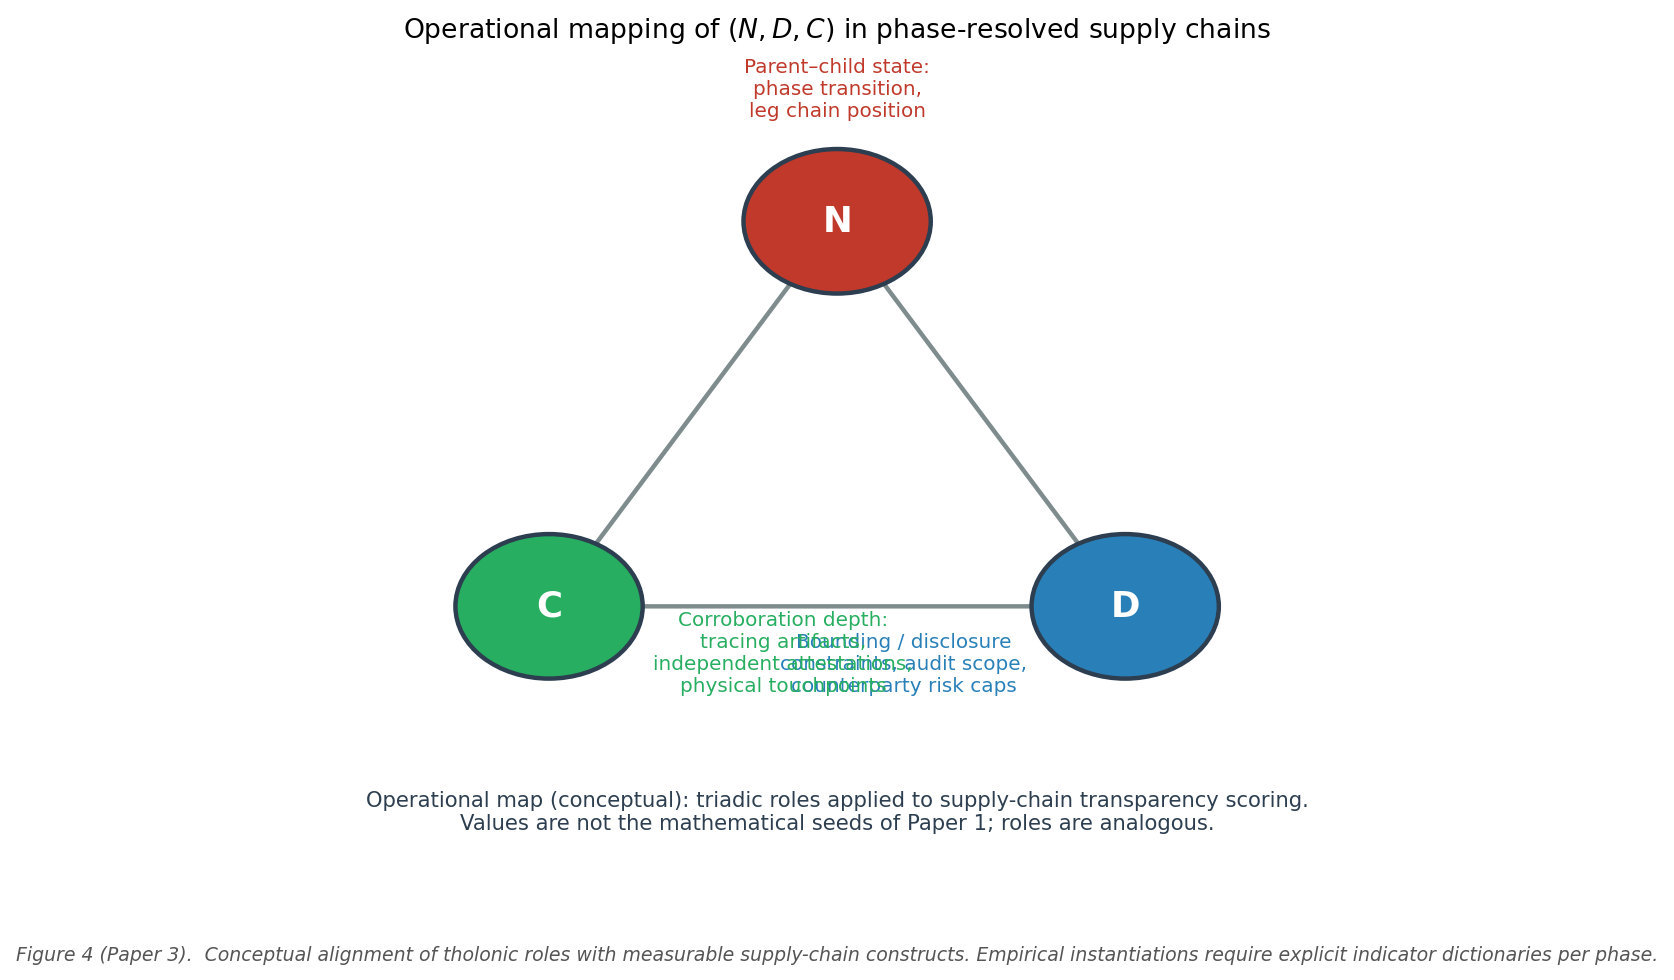
\includegraphics[width=0.80\textwidth]{figures/2_ndc-operational-map}
  \caption{Conceptual map of the three indicator roles $(N_p, D_p, C_p)$ at a supply
           chain phase node.  $N_p$ captures the declared state and its internal
           coherence; $D_p$ bounds the claim; $C_p$ corroborates it independently.}
  \label{fig:ndc-map}
\end{figure}

\subsection{Specimen indicator dictionary (gold, phases 0 and 2)}

An indicator dictionary fixes the mapping from raw evidence items to $(N_p, D_p, C_p)$
values.  The tables below provide a specimen for two phases; a complete deployment
requires entries for all eight phases.

\textbf{Phase~0 (Extraction):}

\begin{table}[ht]
\centering
\caption{Specimen indicators for Phase~0 (Extraction).\label{tab:dict-p0}}
\renewcommand{\arraystretch}{1.15}
\begin{tabular}{>{\raggedright\arraybackslash}p{6.5cm} c >{\raggedright\arraybackslash}p{5cm}}
\toprule
Indicator & Role & Scoring rule (schematic) \\
\midrule
Mass-in / mass-out ratio within 2\% & $N$ & $+20$ if within tolerance \\
Lot number traceable to mining permit & $N$ & $+15$ if traceable; $+8$ if partial \\
Written environmental / social policy exists & $D$ & $+20$ if substantive; $+8$ if nominal \\
Counterparty identity verified (KYC) & $D$ & $+20$ if documented \\
Independent field visit within 12 months & $C$ & $+25$ if within window \\
Geospatial trace & $C$ & $+20$ if available \\\bottomrule
\end{tabular}
\end{table}

\textbf{Phase~2 (Refining):}

\begin{table}[ht]
\centering
\caption{Specimen indicators for Phase~2 (Refining).\label{tab:dict-p2}}
\renewcommand{\arraystretch}{1.15}
\begin{tabular}{>{\raggedright\arraybackslash}p{6.5cm} c >{\raggedright\arraybackslash}p{5cm}}
\toprule
Indicator & Role & Scoring rule (schematic) \\
\midrule
Input mass vs.\ output mass within 0.5\% & $N$ & $+25$ if within tolerance \\
Lot continuity from phase~1 to phase~2 & $N$ & $+20$ if continuous \\
LBMA GDL or equivalent listing \cite{LBMA2021} & $D$ & $+30$ if listed \\
Published responsible sourcing policy & $D$ & $+15$ if substantive \\
Third-party purity certificate & $C$ & $+30$ if from accredited lab \\
Chain-of-custody cross-matched to registry & $C$ & $+20$ if matched \\\bottomrule
\end{tabular}
\end{table}

Scoring rules are \textbf{additive up to a cap of 100}; the cap enforces the $[0,100]$
range without requiring a precise probabilistic interpretation.  Final scale and weights
within each role must be pre-registered before data collection to limit researcher
degrees of freedom.

\begin{remark}[Role distinctness]
Two indicators may share numerical values in a particular chain; what the triadic
structure requires is that \emph{families} of indicators remain functionally distinct.
An operator can maximize $D_p$ without any improvement to $C_p$ (by writing stronger
policies with no independent verification), and vice versa.  The balance functional in
\S\ref{sec:scoring} penalizes this one-sided optimization.
\end{remark}

\section{Scoring model}\label{sec:scoring}

\subsection{Phase-local balance}

Define the \textbf{balance score}
\[
  B_p \;=\; 100\exp\!\left(-\,\frac{2\,|D_p - C_p|}{\max(D_p,\,C_p) + \varepsilon}\right),
\]
where $\varepsilon > 0$ is a small regularization constant.
Properties: (i)~$B_p = 100$ iff $D_p = C_p$; (ii)~$B_p$ is symmetric in $D_p$ and $C_p$;
(iii)~for fixed ratio $r = D_p/C_p$, $B_p$ depends only on the relative imbalance;
(iv)~$B_p \to 0$ as the imbalance ratio grows.
The exponential form guarantees $B_p > 0$ for any finite observables.  The penalty
grows more steeply than linear for imbalance $|D - C|/\max(D,C) > 0.3$ while
remaining forgiving near the diagonal.

\begin{figure}[ht]
  \centering
  \includegraphics[width=0.82\textwidth]{figures/2_balance-metric-B}
  \caption{Balance surface $B(D,C)$ as a function of $(D_p, C_p) \in [0,100]^2$.
    The $D = C$ diagonal achieves $B = 100$; scores fall symmetrically as imbalance grows.}
  \label{fig:balance-surface}
\end{figure}

\subsection{State quality mapping}

Let $g\colon [0,100] \to [0,100]$ map phase state $N_p$ to a quality score.
The simplest case is $g(x) = x$ (the identity).  More complex mappings, such as
threshold-sigmoid functions treating $N_p < 30$ as near-zero quality, are admissible
and must be declared in advance.  For all synthetic examples here, $g = \mathrm{id}$.

\subsection{Transition penalty}

Let $\mathrm{RF}(N_p, N_{p-1}) \geq 0$ be a \textbf{red-flag functional} that increases
when the state claim entering phase $p$ is inconsistent with the state leaving phase $p-1$.
Concrete instances: the absolute mass-balance discrepancy normalized to phase-$(p-1)$
output mass, or the count of identifier mismatches between consecutive phases.  The
\textbf{transition penalty} is
\[
  \tau_p \;=\; \tanh\!\bigl(\,\alpha \cdot \mathrm{RF}(N_p,\,N_{p-1})\bigr),
\]
with $\alpha > 0$ scaling sensitivity.  Since $\tanh$ is bounded, $\tau_p \in [0,1)$.
For the first phase, $\tau_0 = 0$.

\subsection{Aggregate index}

Let $w_p > 0$ with $\sum_{p=0}^{P} w_p = 1$ be phase weights.  The
\textbf{TVPCI aggregate} is
\[
  \mathrm{TVPCI} \;=\; \sum_{p=0}^{P} w_p
  \cdot \Bigl(\beta\,B_p + (1-\beta)\,g(N_p)\Bigr)
  \cdot \bigl(1 - \gamma\,\tau_p\bigr),
\]
where $\beta \in (0,1)$ weights balance against state quality and $\gamma \in (0,1)$
scales the transition-penalty discount.  The product form ensures a high penalty at
phase $p$ reduces that phase contribution without affecting other phases.
The constants $(\beta, \gamma, \alpha, w_p)$ must be \textbf{declared ex ante}.

\textbf{Monotonicity.}  If $D_p = C_p$ and $\tau_p = 0$ for all $p$, then
$\mathrm{TVPCI} = \sum_p w_p N_p$, the weighted average of state scores.  Balance
and penalty terms can only reduce the index; it is monotonically increasing in
$B_p$, $g(N_p)$, and $(1-\tau_p)$.

\textbf{Range.}  $\mathrm{TVPCI} \in [0,100]$ since $B_p, g(N_p) \in [0,100]$ and
$1 - \gamma\tau_p \in (0,1]$ for $\gamma \in [0,1)$.

\textbf{Parameter count.}  For $P+1$ phases the model has $P + 3$ unconstrained
free parameters plus the indicator dictionary.  For $P = 7$ this gives ten free
parameters, manageable if controlled through pre-registration and sensitivity reporting.

\section{Worked numerical example}\label{sec:worked}

We apply the aggregate formula to three representative phases from the synthetic gold
chain: phase~0 (extraction), phase~2 (refining), and phase~7 (exchange anchor).
Parameters: $\beta = 0.5$, $\gamma = 0.5$, $\alpha = 1.0$; weights $w_0 = 0.20$,
$w_2 = 0.35$, $w_7 = 0.45$ (downstream phases receive higher weight, reflecting greater
commercial relevance).

\begin{table}[ht]
\centering
\caption{Worked three-phase TVPCI computation on the synthetic gold baseline.
  A full computation uses all eight phases.\label{tab:worked}}
\renewcommand{\arraystretch}{1.2}
\begin{tabular}{r r r r r r r r r}
\toprule
Phase & $D_p$ & $C_p$ & $N_p$ & $B_p$ & $\mathrm{RF}_p$ & $\tau_p$ & $w_p$ & Contribution \\
\midrule
0 & 18 & 12 & 22 & 74.1 & 0.00 & 0.000 & 0.20 & 9.61 \\
2 & 55 & 58 & 52 & 97.9 & 0.15 & 0.149 & 0.35 & 26.08 \\
7 & 94 & 93 & 90 & 99.5 & 0.02 & 0.020 & 0.45 & 42.81 \\
\midrule
\multicolumn{8}{r}{\textbf{TVPCI}} & \textbf{78.5} \\\bottomrule
\end{tabular}
\end{table}

Phase~0 contributes little because its observables are low (extraction is genuinely
hard to observe) and its weight is lower.  Phase~2 contributes substantially despite
carrying a transition penalty from a small mass-balance anomaly.  Phase~7 contributes
most, reflecting both high local scores and dominant phase weight.

\begin{figure}[ht]
  \centering
  \includegraphics[width=0.88\textwidth]{figures/2_worked-example}
  \caption{Step-by-step TVPCI computation for the three-phase synthetic example,
           showing the phase contributions and the aggregate score of 78.5.}
  \label{fig:worked-example}
\end{figure}

\section{Synthetic comparison and sensitivity analysis}\label{sec:sensitivity}

\subsection{Two-commodity comparison}

Synthetic profiles for gold and shea oil are constructed by choosing phase baselines
that reflect qualitative differences in chain observability: gold benefits from
standardized assay procedures and listed-exchange endpoints; shea oil has a less
formalized upstream (largely artisanal collection) but well-documented refinery and
cosmetics-industry quality standards.  The shea profile is therefore lower at phases~0
and~1, converging toward (but not reaching) the gold profile by phase~7.

Both profiles carry 90\% bootstrap confidence intervals derived by adding normally
distributed indicator noise to each phase baseline (standard deviations ranging from
2 to 7 points), resampled 2\,000 times.  These intervals illustrate \emph{sensitivity
to indicator measurement error}, not empirical sampling variability from a real dataset.

\begin{figure}[ht]
  \centering
  \includegraphics[width=0.90\textwidth]{figures/2_synthetic-transparency-by-phase}
  \caption{Synthetic TVPCI profiles for gold and shea oil with 90\% bootstrap
    confidence intervals.  The gold curve crosses the 50-point illustrative threshold
    at phase~2 (refining); the shea curve crosses it at phase~4.  Intervals narrow at
    phase~7, reflecting lower assumed indicator noise at exchange-anchored endpoints.}
  \label{fig:synthetic-profiles}
\end{figure}

Key observations: (i)~Phase~1 shows the largest absolute gap between commodities
(roughly 10 points) because artisanal shea collection has fewer standardized custody
events than small-scale gold mining subject to conflict-minerals reporting;
(ii)~the gold curve crosses the 50-point illustrative threshold at phase~2 (refining),
the shea curve at phase~4; (iii)~both curves narrow in confidence interval at phase~7,
reflecting the lower indicator noise assumed at exchange-anchored endpoints.

\subsection{Sensitivity to $\beta$ and $\gamma$}

A well-calibrated TVPCI should not change its ordinal ranking of chains substantially
when $\beta$ and $\gamma$ are varied within plausible ranges.  The sensitivity surface
below shows the aggregate score on the synthetic gold baseline as $\beta$ varies from
0 to 1 and $\gamma$ from 0 to 1.

\begin{figure}[ht]
  \centering
  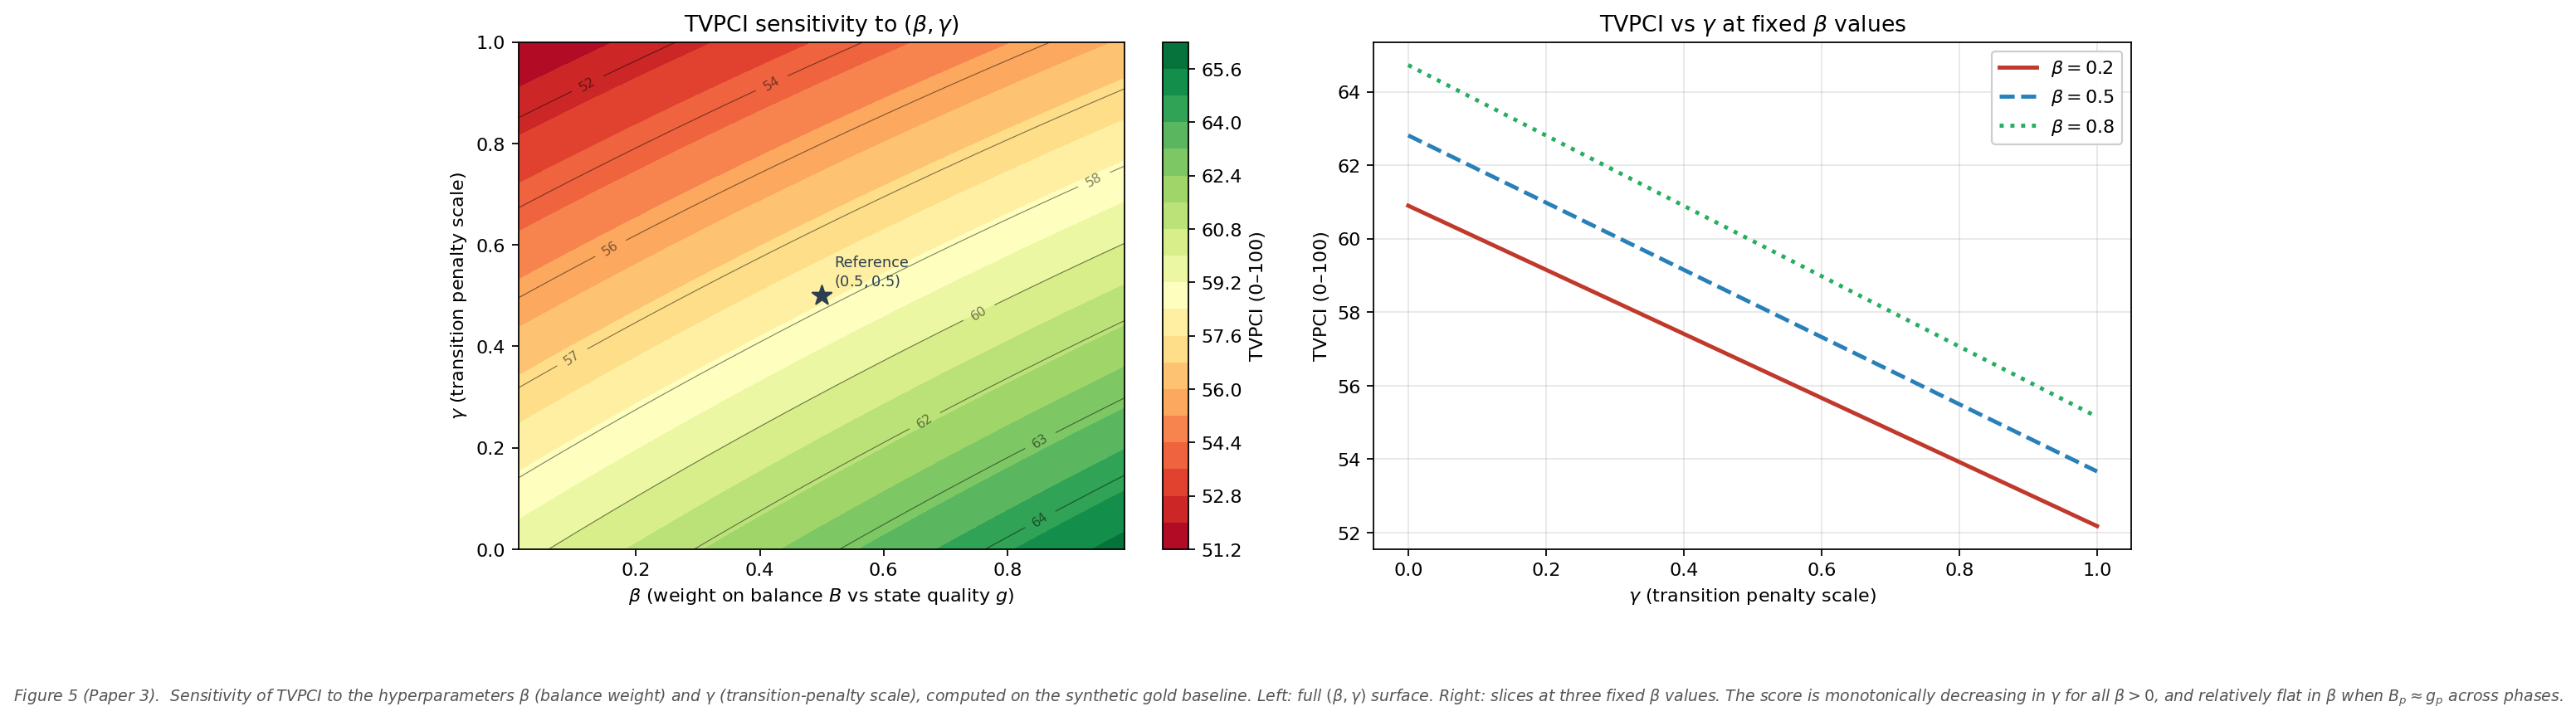
\includegraphics[width=0.85\textwidth]{figures/2_sensitivity-surface}
  \caption{TVPCI sensitivity surface over hyperparameters $(\beta, \gamma)$ on the
    synthetic gold baseline.  Scores are monotonically decreasing in $\gamma$ for all
    $\beta$.  Maximum score variation across the full parameter space is approximately
    8 points.}
  \label{fig:sensitivity-surface}
\end{figure}

Observations: (i)~the score is monotonically decreasing in $\gamma$ for all $\beta$,
confirming that stronger transition penalties uniformly reduce the aggregate;
(ii)~the score is nearly flat in $\beta$ for this synthetic chain, because
$B_p \approx g(N_p)$ across most phases; (iii)~the maximum score variation across the
full parameter space is approximately 8 points.  For chains with larger imbalances,
$\beta$ sensitivity would be substantially higher.  This motivates reporting the
sensitivity surface alongside any published TVPCI calibration.

\section{Discussion}\label{sec:discussion}

\subsection{Organizational vs.\ predictive claims}

TVPCI is an \emph{organizational} instrument: it specifies how to aggregate evidence
into a phase-resolved score.  It does not claim that a score above a threshold guarantees
absence of fraud, conflict sourcing, or human-rights violations.  Those predictive claims
require labeled outcome data and prospective validation.  Framing TVPCI as a scoring
schema rather than a classifier avoids overstating its current evidential status.

\subsection{Post-hoc flexibility and pre-registration}

Any multi-parameter index with analyst discretion over weights and indicator definitions
risks being optimized to produce a desired result.  TVPCI addresses this through three
mitigations.  First, indicator dictionaries and all parameters must be frozen before
observing chain data; any change must be documented as a model revision.  Second,
sensitivity surfaces over $(\beta, \gamma)$ must be published alongside point estimates.
Third, a held-out commodity provides a partial out-of-sample check; if the model was
calibrated on gold, shea oil provides a structural generalization test.

\subsection{Score stability and Lipschitz bounds}

An index score is operationally useful only if small changes in indicators produce small
changes in the aggregate.  Let $\delta_p = (\delta N_p, \delta D_p, \delta C_p)$ be a
perturbation at phase $p$ with $\|\delta_p\|_\infty \leq \epsilon$.  Since $B_p$ is
Lipschitz in $(D_p, C_p)$ (the exponential function has bounded derivative for bounded
inputs) and $g$ is Lipschitz by assumption, the aggregate changes by at most
$O(P\epsilon)$ under small perturbations.  Making this Lipschitz bound explicit would
allow an auditor to certify that a score of, say, 72 is robust to indicator measurement
error of $\pm 3$ points.

\subsection{Missing phases and phase skipping}

Chains lacking documented evidence for an intermediate phase present a practical
challenge.  The proposed convention treats a skipped phase as having maximum imbalance
($B_p \approx 0$) and no state contribution.  If there is positive reason to believe
the phase was uneventful, a less aggressive default may be adopted, but must be
pre-registered as a modeling choice.

\subsection{Legal and jurisdictional definitions}

Several indicators in the specimen dictionary refer to legal concepts (origin,
conflict-affected area, KYC documentation) that are jurisdiction-specific.  A global
deployment of TVPCI would require jurisdiction-specific indicator dictionary variants.
Standardization bodies such as OECD and LBMA could provide a mapping.

\subsection{Regulatory alignment}

Mapping TVPCI to OECD five-step guidance \cite{OECD2016} is feasible.  OECD step~2
(risk identification) corresponds to identifying phases with low $N_p$ or low $B_p$;
step~3 (strategy response) to the action required to raise specific phase scores;
step~4 (third-party audit) to independently verifying the $C_p$ indicators.  A
companion compliance note mapping TVPCI fields to OECD steps and GRI 308/414
disclosures \cite{GRI308,GRI414} would be a useful practical deliverable.

\section{Conclusion}\label{sec:conclusion}

We introduced \textbf{TVPCI}, a phase-resolved transparency scoring framework for
commodity supply chains.  The framework assigns three functionally distinct observables
$(N_p, D_p, C_p)$ to each phase, computes a balance score $B_p$ penalizing one-sided
evidence, and applies transition penalties when chain-state claims are internally
inconsistent across phases.  A weighted aggregate combines these elements into a single
index on $[0, 100]$.

The framework was demonstrated on synthetic eight-phase gold and shea-oil profiles.
Worked numerical examples, sensitivity analysis over $\beta$ and $\gamma$, and a
two-commodity comparison illustrate the scoring machinery.  All presented data are
synthetic.

Immediate next steps for an empirical deployment are:
\begin{enumerate}
  \item Fix indicator dictionaries for one commodity through expert consultation and
        pre-registration.
  \item Apply the schema to real chains with known audit outcomes, using those outcomes
        as a validation signal.
  \item Publish the sensitivity surface and held-out commodity results alongside any
        point estimates.
  \item Develop a Lipschitz stability certificate for the chosen indicator-noise level.
\end{enumerate}

\bibliographystyle{plainnat}
\bibliography{2_supply-chain-transparency-tvpci}

\appendix
\section{Figure checklist}\label{app:figures}

\begin{table}[ht]
\centering
\caption{All figure assets for this paper.  Filenames begin with \texttt{2\_},
  reserved for this paper.\label{tab:figcheck}}
\renewcommand{\arraystretch}{1.15}
\begin{tabular}{ll>{\raggedright\arraybackslash}p{4.5cm}}
\toprule
File & Section & Content \\
\midrule
\texttt{2\_gold-phase-ladder.png} & \S\ref{subsec:gold-phases} & Eight-phase gold ladder \\
\texttt{2\_balance-metric-B.png} & \S\ref{sec:scoring} & Balance surface $B(D,C)$ \\
\texttt{2\_ndc-operational-map.png} & \S\ref{sec:observables} & Indicator-role map \\
\texttt{2\_synthetic-transparency-by-phase.png} & \S\ref{sec:sensitivity} & Two-commodity profiles \\
\texttt{2\_sensitivity-surface.png} & \S\ref{sec:sensitivity} & Hyperparameter surface \\\bottomrule
\end{tabular}
\end{table}

\end{document}
